\documentclass[border=5mm]{standalone}
\usepackage{pgfplots}
\pgfplotsset{compat=1.18}

\begin{document}
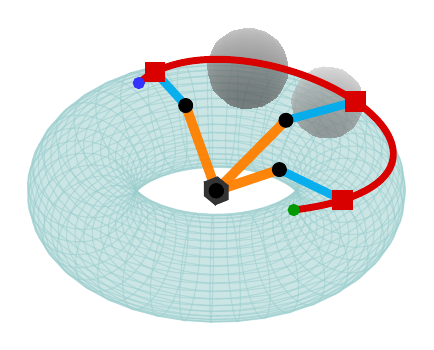
\begin{tikzpicture}
\begin{axis}[
    view={55}{35}, % Ángulo optimizado para la perspectiva 3D
    axis lines=none,
    colormap={mymap}{
        color(0)=(gray!80);           % 0 representa un obstáculo
        color(1)=(teal!60!white);     % 1 representa espacio libre (C_free)
    },
    unit vector ratio=1 1 1,
]
    \def\R{3}   % Radio mayor del toro
    \def\r{1.2} % Radio menor del toro
    \def\LOne{1.8} 
    \def\LTwo{1.5} 

    % 1. Toro C-space (Limpio y Traslúcido)
    \addplot3[
        surf,
        z buffer=sort,
        samples=40,
        domain=0:360,
        y domain=0:360,
        opacity=0.3,
        mesh/rows=40,
        teal!40!white,
        shader=flat
    ] (
        {(\R + \r*cos(y))*cos(x)},
        {(\R + \r*cos(y))*sin(x)},
        {\r*sin(y)}
    );

    % 2. OBSTÁCULOS: Esferas 3D (Bolas en C-space)
    % Obstáculo 1: Posición (90, 90)
    \addplot3[
        surf,
        opacity=0.7,
        samples=15,
        domain=0:360,
        y domain=0:180,
        colormap={blackwhite}{color(0cm)=(black!90); color(1cm)=(gray!30)},
        shader=interp
    ] (
        {0 + 0.8*cos(x)*sin(y)}, 
        {3 + 0.8*sin(x)*sin(y)}, 
        {1.2 + 0.8*cos(y)}
    );
    
    % Obstáculo 2: Posición (135, 30)
    \addplot3[
        surf,
        opacity=0.7,
        samples=15,
        domain=0:360,
        y domain=0:180,
        colormap={blackwhite}{color(0cm)=(black!90); color(1cm)=(gray!30)},
        shader=interp
    ] (
        {-2.8 + 0.9*cos(x)*sin(y)}, 
        {2.8 + 0.9*sin(x)*sin(y)}, 
        {0.6 + 0.9*cos(y)}
    );

    % 3. Trayectoria Espacial (Línea Roja)
    \addplot3[
        domain=0:180,
        samples=80,
        samples y=0,
        line width=2.5pt,
        red!85!black,
    ] (
        {(\R + \r*cos(90 - 60*sin(x)))*cos(x)},
        {(\R + \r*cos(90 - 60*sin(x)))*sin(x)},
        {\r*sin(90 - 60*sin(x))}
    );

    % MACRO: ROBOT CENTRALIZADO
    \newcommand{\drawCentralRobot}[1]{
        \pgfmathsetmacro{\targetX}{(\R + \r*cos(90-60*sin(#1)))*cos(#1)}
        \pgfmathsetmacro{\targetY}{(\R + \r*cos(90-60*sin(#1)))*sin(#1)}
        \pgfmathsetmacro{\targetZ}{\r*sin(90-60*sin(#1))}
        
        \pgfmathsetmacro{\midX}{0.5*\targetX}
        \pgfmathsetmacro{\midY}{0.5*\targetY}
        \pgfmathsetmacro{\midZ}{0.5*\targetZ + 0.7}

        \addplot3[orange, line width=3.5pt, opacity=0.95] coordinates {(0,0,0) (\midX, \midY, \midZ)};
        \addplot3[cyan, line width=3pt, opacity=0.95] coordinates {(\midX, \midY, \midZ) (\targetX, \targetY, \targetZ)};
        \addplot3[only marks, mark=*, mark size=2.5pt, black] coordinates {(0,0,0) (\midX, \midY, \midZ)};
        \addplot3[only marks, mark=square*, mark size=3.5pt, red!85!black] coordinates {(\targetX, \targetY, \targetZ)};
    }

    \addplot3[only marks, mark=cube*, mark size=5pt, black!80] coordinates {(0,0,0)};

    \drawCentralRobot{20}
    \drawCentralRobot{95}
    \drawCentralRobot{170}

    % Puntos clave
    \addplot3[only marks, mark=*, mark size=2pt, green!60!black] coordinates {(\R, 0, \r)};
    \addplot3[only marks, mark=*, mark size=2pt, blue!80!white] coordinates {(-\R, 0, \r)};

\end{axis}
\end{tikzpicture}
\end{document}
